\section{Ejercicio 1}

\subsection{Introducción}

Se tiene un mapa de $N$ esquinas y $M$ calles bidireccionales en donde las esquinas pueden ser casas de alumnos de secundaria, escuelas o esquinas neutrales. El problema consiste en encontrar la mínima cantidad de esquinas en las que podemos podemos poner a un estudiante del departamento a contar sobre la carrera de Ciencias de la Computación, de modo tal que no importe qué camino utilice cada chico para llegar de su casa al colegio, ni a qué colegio vaya cada chico, siempre tenga que pasar por una esquina donde lo podamos interceptar para contarle de la carrera.

\subsection{Solución propuesta}

La resolución de este ejercicio consiste en modelar el mapa como un grafo, y más específicamente como una red de flujo, y obtener el flujo máximo. En esta red de flujo se tiene las casas de los estudiantes conectadas a la fuente y las escuelas al sumidero (pero podría ser al revés y no afectaría en lo absoluto).

Las capacidades de las aristas serán de 1, pero además también deben tener capacidad 1 los nodos. Para modelar las capacidades de los vértices, se representó cada uno de ellos como un arco de capacidad 1 cuyos extremos son un nodo en donde inciden todas las aristas que incidirían en el vértice original y otro con todas las aristan salientes.

\begin{figure}[H]
\centering
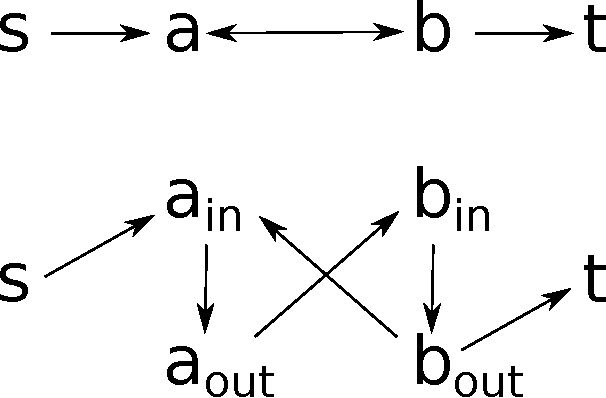
\includegraphics[scale=0.6]{imagenes/ej1_capacidades_nodos.pdf}
\end{figure}

Se construye la red residual y luego se aplica el ya conocido algoritmo de Edmond-Karps para conocer el flujo máximo.

\subsubsection*{Pseudocódigo}

La estructura utilizada para la representación de la red fue un vector de listas de enteros (lista de adyacencias). Se reservaron las dos primeras posiciones del vector para la fuente y el sumidero.

\begin{algorithm}[]
	\caption{flujoMáximo}
	\Input{$Vector<Lista<Entero>>$ $redResidual$}
	\Output{$Entero$ $flujoMaximo$}

	$flujo$ $\gets$ 0 \;
	$Lista<Entero>$ $camino$ $\gets$ BFS($redResidual$, FUENTE, SUMIDERO) \;
	\While{$\neg camino$.vacio()} {
		recorrerCaminoDeAumento($redResidual$, $camino$) \;
		$camino$ $\gets$ BFS($redResidual$, FUENTE, SUMIDERO) \;
		$flujo$ $\gets$ $flujo + 1$ \;
	}
	\Return $flujo$ \;
\end{algorithm}

\begin{algorithm}[]
	\caption{recorrerCaminoDeAumento}
	\Input{$Vector<Lista<Entero>>$ $redResidual$(por referencia), $Lista<Entero>$ $camino$}

	$Iterador<Lista<Entero>>$ $itCamino$ $\gets$ $camino$.Primero() \;
	\While{$itCamino$.siguiente() $\not=$ $camino$.Fin()} {
		Entero $desde$ $\gets$ *$itCamino$ \;
		Entero $hasta$ $\gets$ *($itCamino$.siguiente()) \;
		$redResidual$[$desde$].borrar($hasta$) \;
		$redResidual$[$hasta$].agregar($desde$) \;
		$itCamino$++ \;
	}
\end{algorithm}

Notar que en recorrerCaminoDeAumento se borran y agregan aristas porque las capacidades de las mismas son siempre 1. De lo contrario habría que tenerse en cuenta la capacidad de las mismas, no se borrarían y agregarían sino que se aumentaría o restaría el flujo que pasa por el eje.

\subsection{Correctitud}

Lo que el algoritmo debe devolver es la minima cantidad de esquinas a donde puedan situarse estudiantes de modo tal que cada alumno de secundaria siempre tenga que pasar por una de estas esquinas sin importar que camino tome o a que colegio vaya.

En otras palabras, existen conjuntos de esquinas para los cuales todos los caminos de las casas a las escuelas pasan por al menos una de las esquinas del conjunto. El que interesa es el de mínimo cardinal (un conjunto que tenga todas las esquinas por supuesto que cumpliría el requisito de interceptar los alumnos, pero no sería mínimo).

Este conjunto de mínimo cardinal representa un cuello de botella en cuanto a los caminos que los alumnos de secundaria pueden elegir.

Lo que el algoritmo devuelve es el valor flujo máximo. Por teorema se sabe que el valor del flujo máximo es igual a la capacidad del corte mínimo.

Lo que hace que la capacidad del corte mínimo en esta red de flujo represente el cardinal del conjunto de esquinas es el hecho de que los vértices tengan capacidad 1. Esto provoca que la capacidad del corte no este dada por la capacidad de las aristas salientes sino por la cantidad de nodos del corte que tienen aristas salientes. Entonces si para cualquier corte de esta red de flujo, su capacidad es igual a la cantidad de nodos con aristas salientes, es decir, esquinas de las cuales salen caminos, consiguiendo el corte mínimo se obtendría el cuello de botella y su capacidad sería el cardinal del conjunto.

Entonces el valor del flujo máximo de esta red es la mínima cantidad de esquinas en las que deben situarse estudiantes para poder interceptar a todos los alumnos sin importar qué caminos tomen o a qué escuela asistan.